\section{Sensor characterisaton}
The simplest method to calibrate the SiPMs is shown in figure \ref{fig:calibration} (top panel), and consists  in finding the different peaks associated to the different photoelectron numbers in the SiPM and extract the gain according to their separation. The first results from NEW show that the gain spread among the SiPMs is very small (figure \ref{fig:calibration} bottom).
%The first data extracted from the tracking plane has been used to make a first evaluation of the behaviour of the different sensors and DICE boards. The SiPMs have been tested with no light (only dark counts were recorded) and with light pulses from the blue LEDs installed in the energy plane (Fig. \ref{fig:calibration} bottom).

\begin{figure}[h!]
\centering
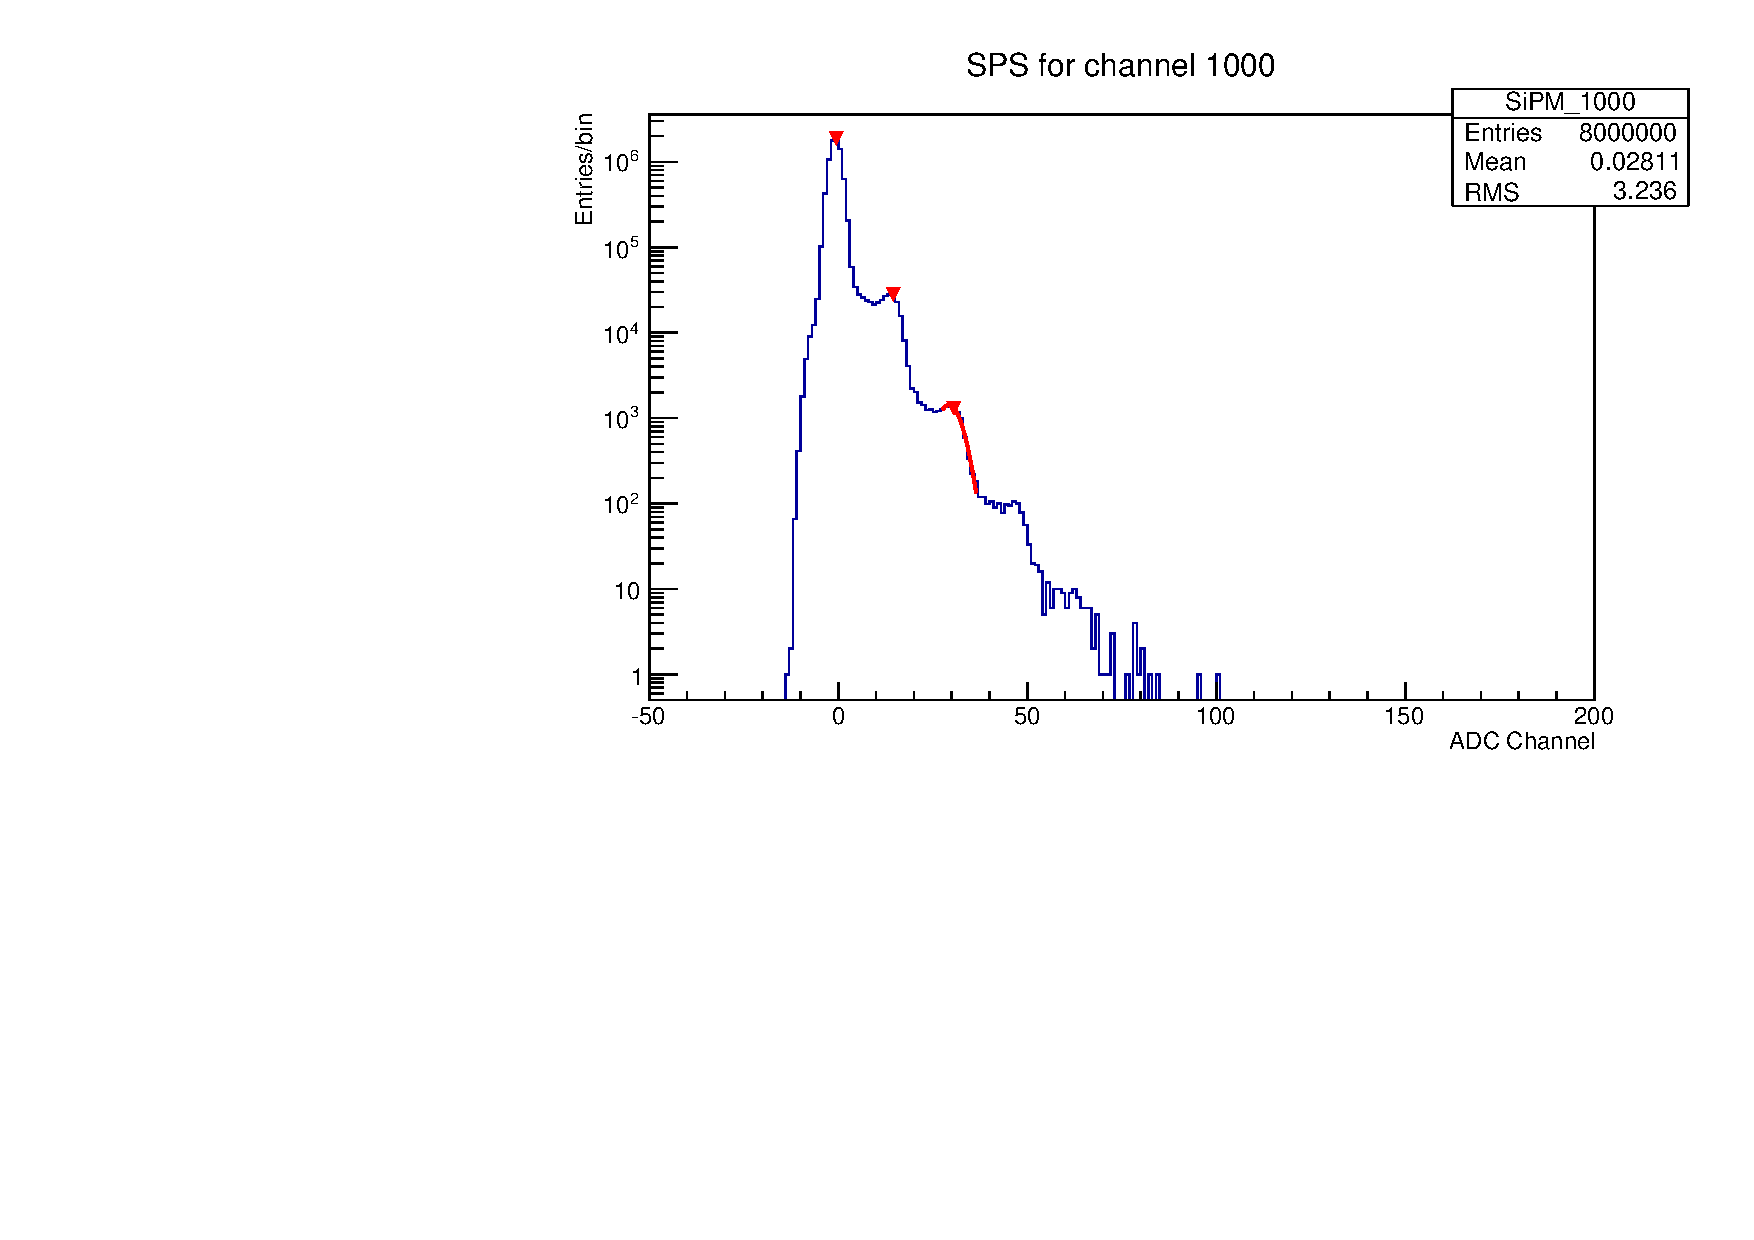
\includegraphics[width=0.45\textwidth]{IMG/normal_calibration}
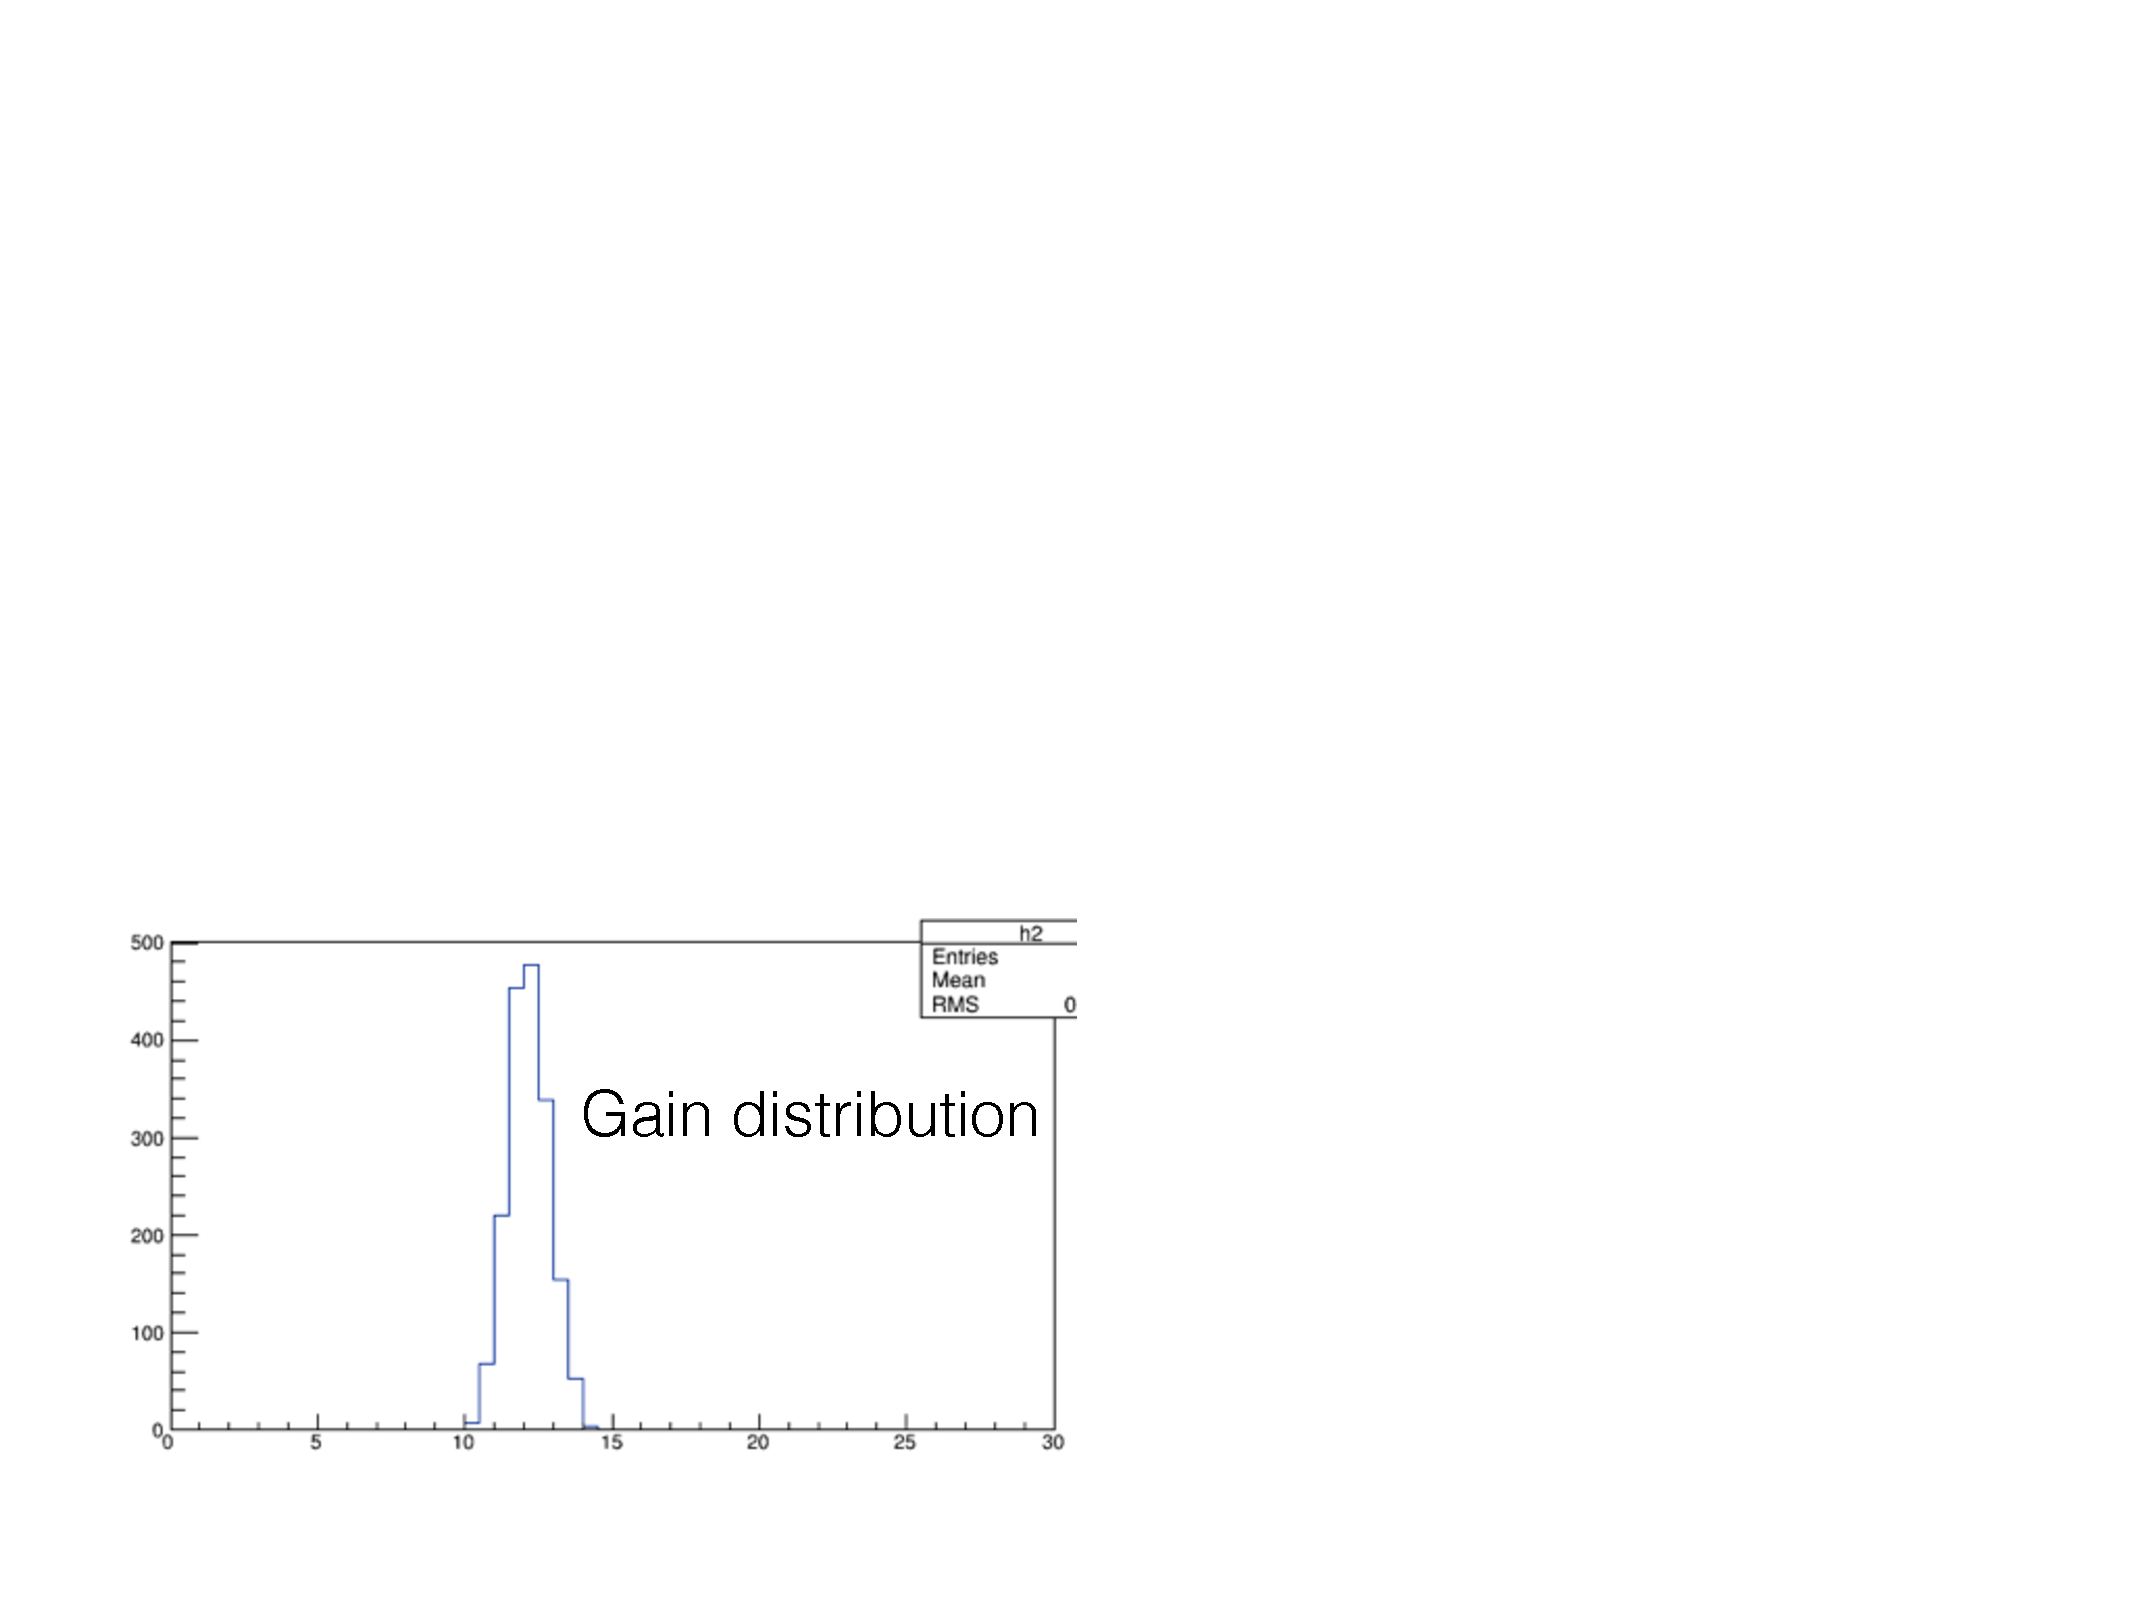
\includegraphics[width=0.45\textwidth]{IMG/SIPMsGain}
%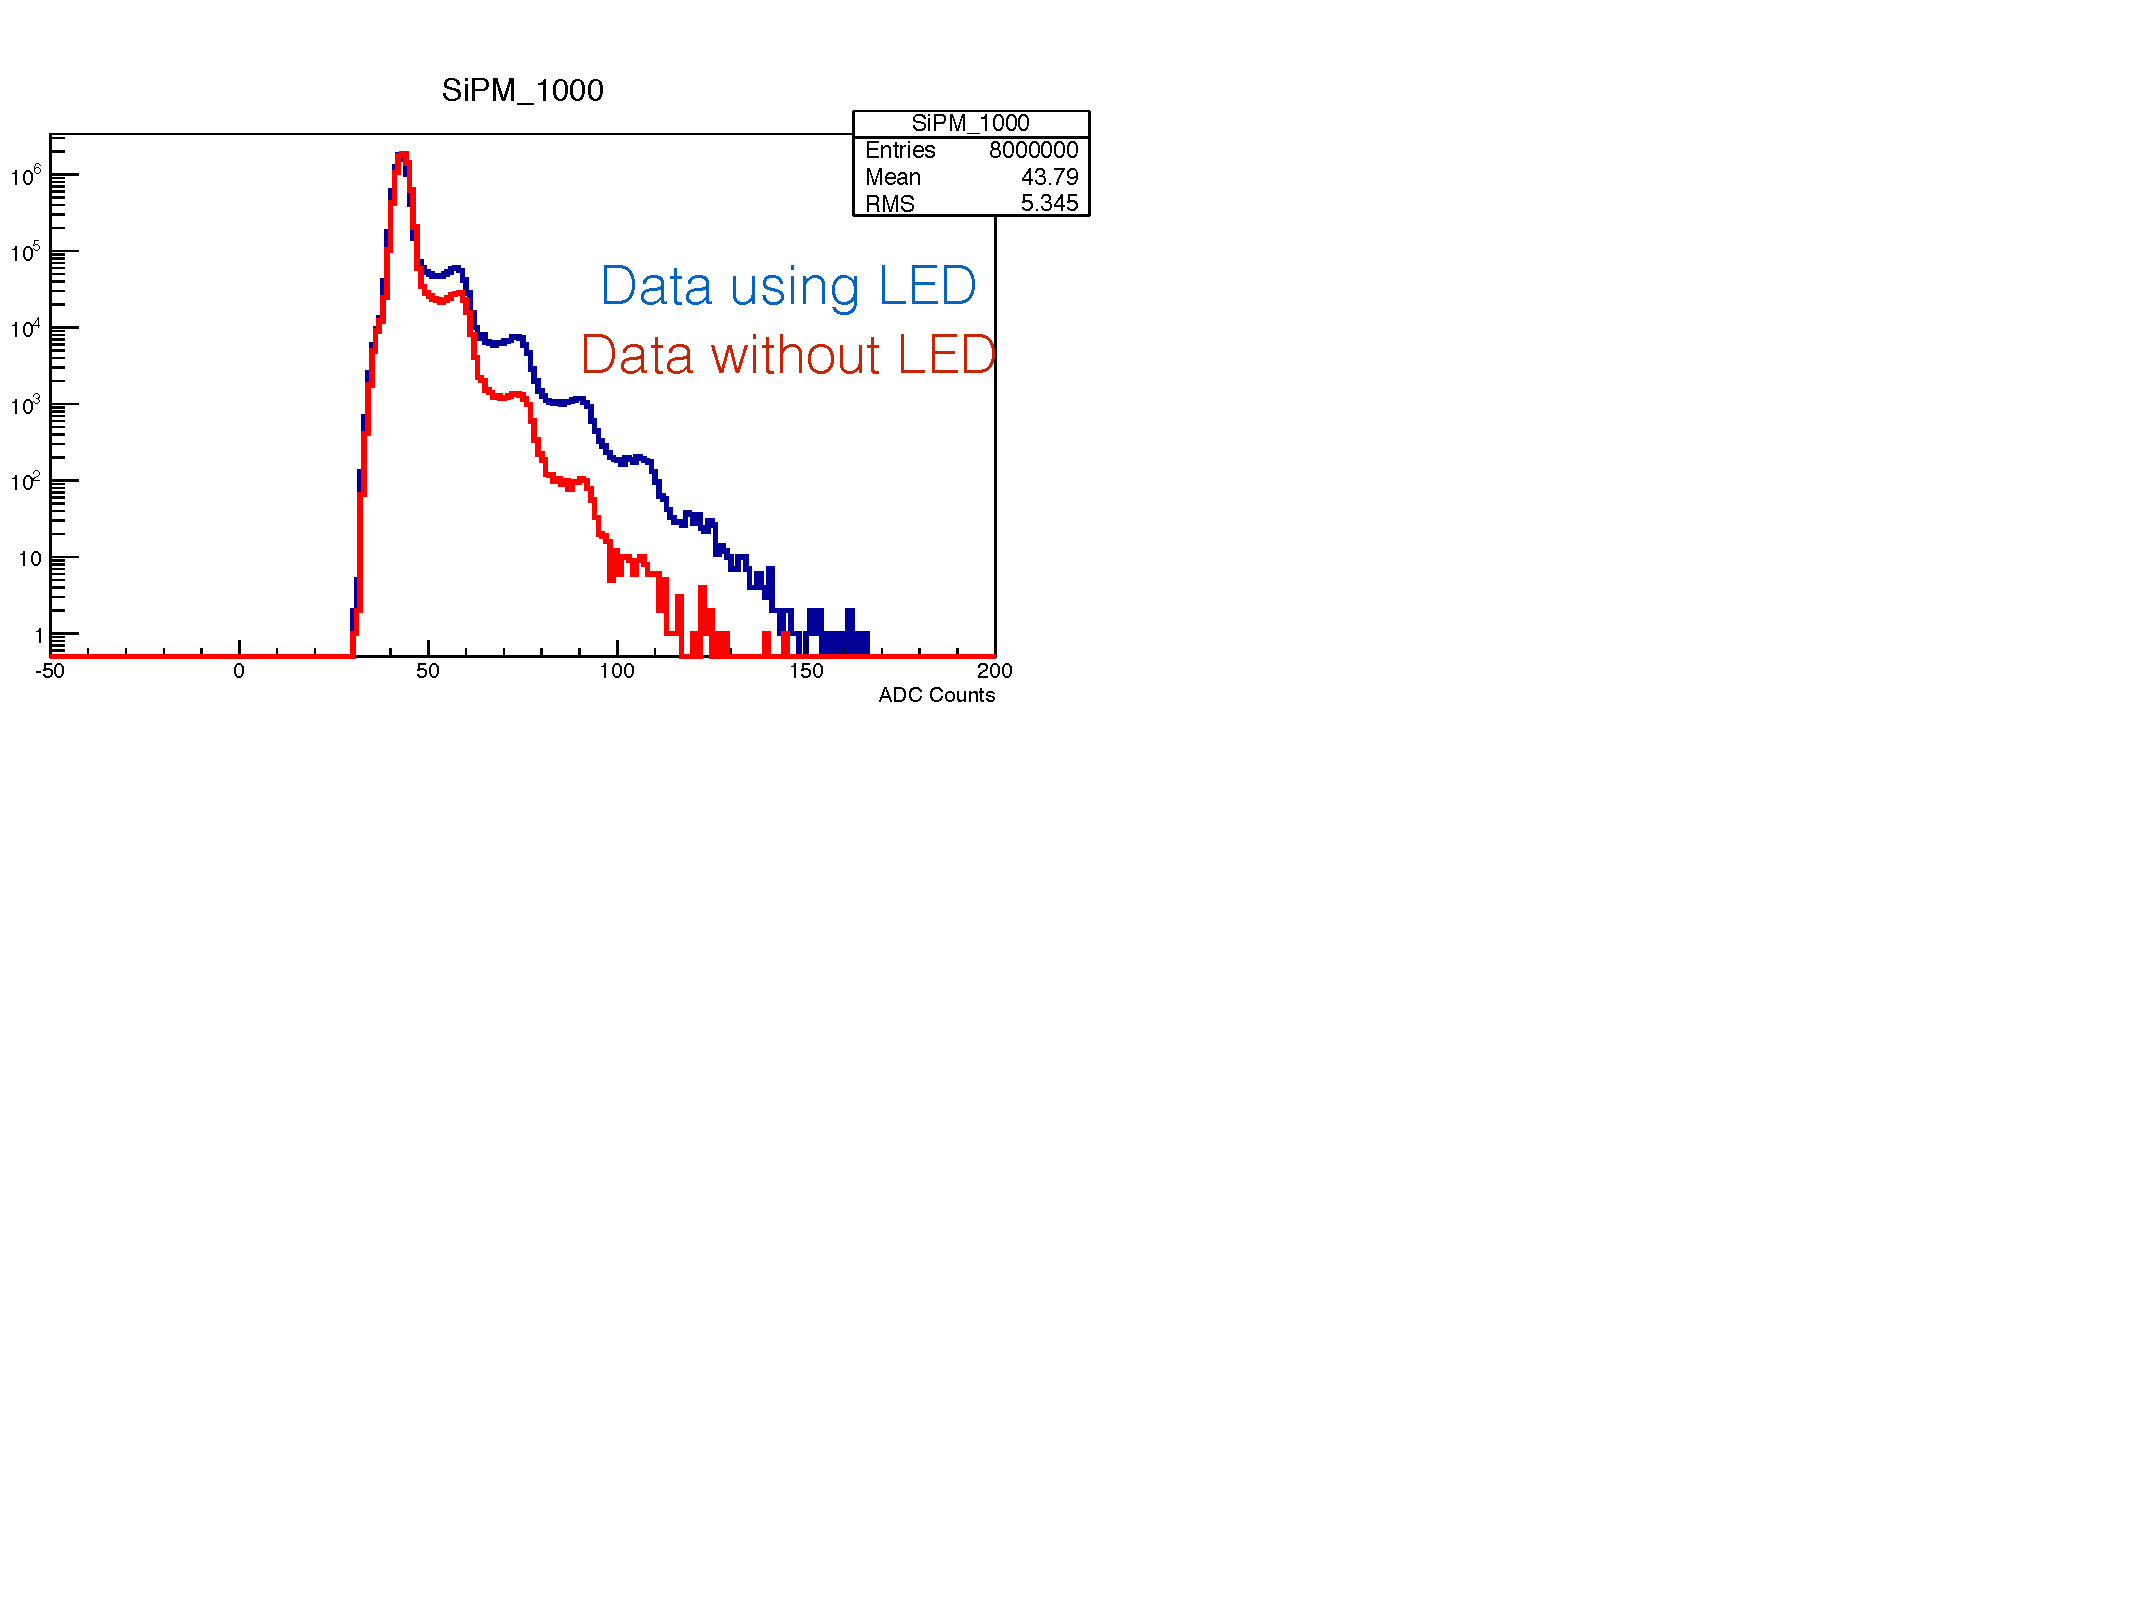
\includegraphics[width=0.45\textwidth]{IMG/SiPM_LED_noLED}
\caption{Top: standard method for calibration where the charge corresponding to the different number of photoelectrons in the SiPMs is estimated with a fit to the peak. The gain of the SiPM is calculated using the separation of the different peaks. Bottom: Histogram showing the gain of all the SiPMs in the plane. This histogram shows that the spread on the SiPMs gain is only of the order of a few ADC counts. 
%Bottom: Comparison of two spectra from the same SiPM, with (blue) and without light (red).
}
\label{fig:calibration}
\end{figure}

%Different methods for calibrating the SiPMs are currently being tested. The simplest method is based in a finding the different peaks associated to the different photoelectron number in the SiPM extract the gain according to their separation (Fig. \ref{fig:calibration} up left). This method was the one used in NEXT-DEMO and has demonstrated good performance. The first results show that the gain spread among the SiPMs is very small (Fig. \ref{fig:calibration} up right). However, some other methods may give a better characterization of the SiPMs that will include the integral effect of the dark count, quantum efficiency and cross-talk. Those other methods are being tested.